\section{Geometry}

\subsection{Trigonometry}

\begin{equation}
  \sin(v+w)=\sin v\cos w+\cos v\sin w
\end{equation}

\begin{equation}
  \cos(v+w)=\cos v\cos w-\sin v\sin w
\end{equation}

\begin{equation}
  \tan(v+w)=\dfrac{\tan v+\tan w}{1-\tan v\tan w}
\end{equation}

\begin{equation}
  \sin v+\sin w=2\sin\dfrac{v+w}{2}\cos\dfrac{v-w}{2}
\end{equation}

\begin{equation}
  \cos v+\cos w=2\cos\dfrac{v+w}{2}\cos\dfrac{v-w}{2}
\end{equation}

\begin{equation}
\begin{array}{c}
 (V+W)\tan(v-w)/2{}=(V-W)\tan(v+w)/2 \\
  \text{where $V, W$ are lengths of sides opposite angles $v, w$.}
\end{array}
\end{equation}


\begin{equation}
\begin{array}{c}
	a\cos x+b\sin x=r\cos(x-\phi) \\
	a\sin x+b\cos x=r\sin(x+\phi) \\
  \text{where $r=\sqrt{a^2+b^2}, \phi=\operatorname{atan2}(b,a)$.}
\end{array}
\end{equation}

 


\subsection{Line}

\subsubsection{General equation}

\begin{equation}
    ax + by + c = 0
\end{equation}

Note that a same line can have multiple representations (just multiply the equation by any real number), so to make each line have a single equation divide everyhting by $a$, or $b$ if $a$ is zero.

\subsubsection{General equation from two points}

Let $P$ and $Q$ be the points that define the line.

\[
  \begin{array}{l}
  a = P_y - Q_y \\
  b = Q_x-P_x  \\
  c = P \times Q = P_x Q_y - P_y Q_x \\
  \end{array}
\]


\subsubsection{Line inclination from two points}

Let $P$ and $Q$ be two points that belongs to the line, such that $P_x < Q_x$ the inclination $m$ or angular coefficient is given by:

\begin{equation}
    m = \frac{Q_y - P_y}{Q_x - P_x}
\end{equation}

\subsubsection{Check if a point belongs to the line}

Let $r$ be a line such that $ax + by + c = 0$ and $P$ a point. $P \in r$ if and only if :

\[
  a P_x + b P_y + c = 0
\]

\subsubsection{Distance from a point to a line}

The distance from a point $P$ and a line $r$ is defined as the shortest distance possible between every point that belongs to $r$ and $P$. Such distance will be the distance from $P$ and the intersection between $r$ and the orthogonal projection from $P$ to $r$, and can be found by:


\[
    \frac{|a P_x + b P_y +c|}{\sqrt{a^2+b^2}}
\]

The coordinates of the point $Q$ are given by:

\[
  \begin{array}{c}
    Q_x = \frac{b (b P_x - a P_y)-ac}{a^2+b^2} \\
    Q_y = \frac{a(-bP_x+aP_y)-bc}{a^2+b^2} \\
  \end{array}
\]




\subsection{Convex and Concave Polygons}


\begin{figure}[H]
    \centering
    \begin{minipage}[b]{0.25\textwidth}
        \centering
        \includegraphics[width=\linewidth]{media/Convex-Polygon.jpg}
        \caption{Convex Polygon}
    \end{minipage}%
    \begin{minipage}[b]{0.25\textwidth}
        \centering
        \includegraphics[width=\linewidth]{media/Concave-Polygon.jpg}
        \caption{Concave Polygon}
    \end{minipage}
    \caption{Two Types of Polygons}
\end{figure}

\subsubsection{Regular polygon circumradius}

    \def\R{3}

    \begin{figure}[H]
        \centering
        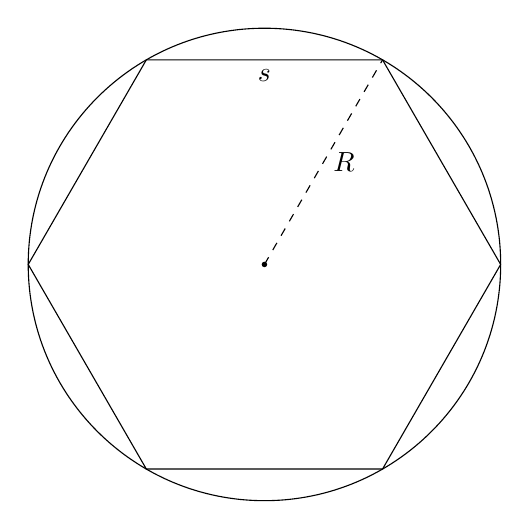
\begin{tikzpicture}
            \draw (0:\R) -- (60:\R) -- node[anchor=north] { $s$ } (120:\R) -- (180:\R) -- (240:\R) -- (300:\R) -- (360:\R) -- (0:\R);
            \draw (0, 0) circle [radius=\R];
            \fill (0, 0) circle [radius=1pt];
            \draw[dashed] (0, 0) -- node[anchor=west] { $R$ } (60:\R);

        \end{tikzpicture}
    \end{figure}

    \[
        R = \frac{s}{2}\csc\frac{\pi}{n}
    \]

\subsubsection{Regular polygon inscribed circle radius}

    \def\R{3}

    \begin{figure}[H]
        \centering
        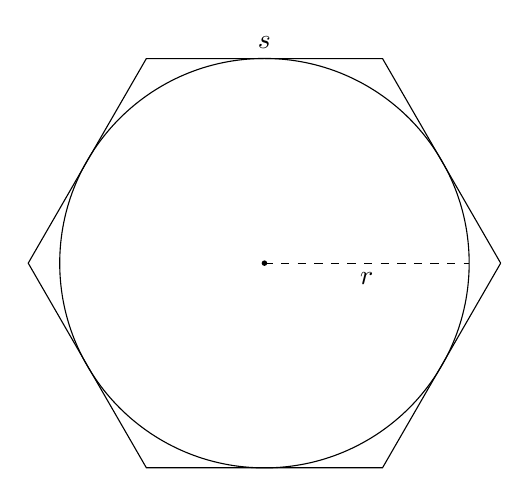
\begin{tikzpicture}
            \draw (0:\R) -- (60:\R) -- node[anchor=south] { $s$ } (120:\R) -- (180:\R) -- (240:\R) -- (300:\R) -- (360:\R) -- (0:\R);
            \draw (0, 0) circle [radius=2.6];
            \fill (0, 0) circle [radius=1pt];
            \draw[dashed] (0, 0) -- node[anchor=north] { $r$ } (2.6, 0);

        \end{tikzpicture}
    \end{figure}

        \[
        r = R\cos \frac{\pi}{n}
        \]



\subsubsection{Area of regular polygons}

    \begin{itemize}
        \item Let $n$ be the number of sides of the regular polygon, the area can be found using one of the values below:
            \begin{enumerate}
                \item  the lenght of one of the sides ($s$)
                \item apothem, the radius of the inscribed circle ($r$)
                \item the radius of the circumscribed circle ($R$)
            \end{enumerate}

        \[
            A = \frac{1}{2}nrs = \frac{1}{4}ns^2\cot \frac{\pi}{n} = nr^2\tan \frac{\pi}{n} = \frac{1}{2}nR^2\sin \frac{2\pi}{n}
        \]

    \end{itemize}


\subsubsection{Sum of internal angle of a regular polygon}
A regular polygon with $n$ sides have $(n-2)180$ degrees as sum of it's internal angle.



\subsection{Triangle}

Let the lenght of the sides of the triangle be $a$, $b$, $c$.

\subsubsection{Semiperimeter}

Let $p$ be the semiperimeter definded as: 

\begin{equation}
  p = \frac{a + b + c}{2}
\end{equation}

\subsubsection{Area}

Let $A$ be the area defined as:

\begin{equation}
  \sqrt{p(p-q)(p-b)(p-c)}
\end{equation}

\subsubsection{Circumradius}

\begin{equation}
  R = \frac{abc}{4A}
\end{equation}

\subsubsection{Inradius}

\begin{equation}
  r = \frac{A}{p}
\end{equation}

\subsubsection{Lenght of bisector}

\begin{equation}
s_a=\sqrt{bc\left[1-\left(\dfrac{a}{b+c}\right)^2\right]}
\end{equation}

\subsubsection{Law of sines}

\begin{equation}
  \dfrac{\sin\alpha}{a}=\dfrac{\sin\beta}{b}=\dfrac{\sin\gamma}{c}=\dfrac{1}{2R}
\end{equation}

\subsubsection{Law of cosines}

\begin{equation}
  a^2=b^2+c^2-2bc\cos\alpha
\end{equation}

\subsubsection{Law of tangents}

\begin{equation}
  \dfrac{a+b}{a-b}=\dfrac{\tan\dfrac{\alpha+\beta}{2}}{\tan\dfrac{\alpha-\beta}{2}}
\end{equation}




\subsection{Quadrilaterals}

Let it's sides lenght be $a,b,c,d$

\subsubsection{Intersection of ... ?}

\begin{figure}[H]
    \centering

    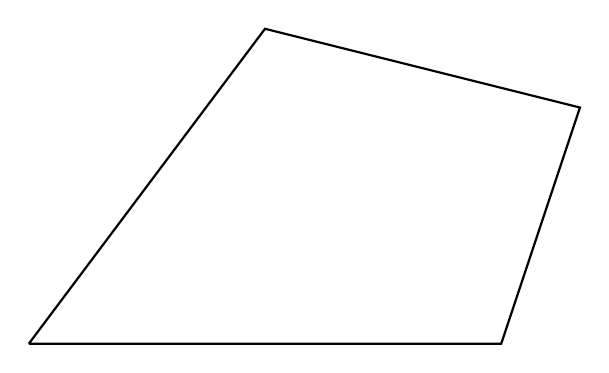
\begin{tikzpicture}
        \coordinate (A) at (0, 0);
        \coordinate (B) at (3, 4);
        \coordinate (C) at (7, 3);
        \coordinate (D) at (6, 0);

        \coordinate (MAB) at (1.5, 2);
        \coordinate (B) at (3, 4);
        \coordinate (C) at (7, 3);
        \coordinate (D) at (6, 0);

        \draw[thick] (A) --  (B) -- (C) -- (D) -- (A);

    \end{tikzpicture}
\end{figure}


\subsection{Trapezium}

\subsubsection{Area}
\begin{figure}
    \centering

    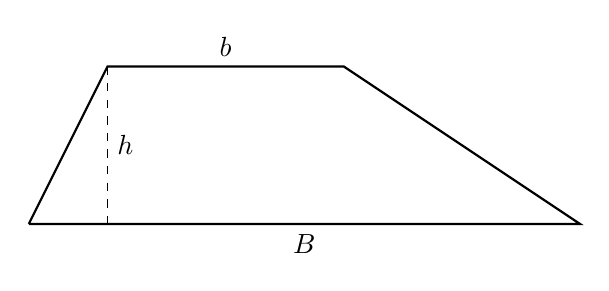
\begin{tikzpicture}
        \coordinate (A) at (0, 0);
        \coordinate (B) at (7, 0);
        \coordinate (C) at (4, 2);
        \coordinate (D) at (1, 2);
        \coordinate (O) at (1, 0);

        \draw[thick] (A) -- node[anchor=north] { $B$ } (B) -- (C) -- node[anchor=south] { $b$ } (D) -- (A);
        \draw[dashed] (D) -- node[anchor=west] { $h$ } (O);

    \end{tikzpicture}
\end{figure}
\[
    A = \frac{(B + b)h}{2}
\]



\subsection{Sphere}

\subsubsection{Equation}

    \[
        (x - x_0)^2 + (y - y_0)^2 + (z - z_0)^2 = r^2
    \]

\subsubsection{Equation in spherical coordinate system}
  $r$ is the radius, $\theta$ is an angle that goes from $0$ to $2\pi$, and $\varphi$ is an angle that goes from $0$ to  $\pi$.
  \[
    \begin{array}{l}
        x = x_0 + r\cos \theta\sin \varphi \\
        y = y_0 + r\sin \theta\sin \varphi \\
        z = z_0 + r\cos \varphi \\
    \end{array}
  \]


\subsubsection{Area}

  $A = 4\pi r^2$, where $r$ is the radius, comes from :

  \[
      A = \int_0^\pi \int_0^{2\pi} r^2\sin(\varphi)\ d\theta d\varphi
  \]
\subsubsection{Volume}

        \[
            V = \frac{4}{3}\pi r^3
        \]
        comes from :

        \[
            V = \int_0^R \int_0^\pi \int_0^{2\pi} r^2\sin(\varphi)\ d\theta d\varphi dR
        \]





\subsection{Cube}

\subsubsection{Facial \& Body diagonal}

Facial diagonal join two vertices at the same face.

Body diagonal join two vertices from opposite faces.

\begin{figure}[H]
  \centering
  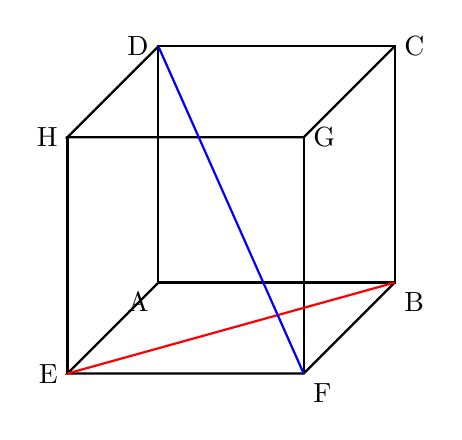
\begin{tikzpicture}[scale=1.5] % Define vertices
    \coordinate (A) at (0,0,0); \coordinate (B) at (2,0,0); \coordinate (C) at (2,2,0); \coordinate (D) at (0,2,0); \coordinate (E) at (0,0,2); \coordinate (F) at (2,0,2); \coordinate (G) at (2,2,2); \coordinate (H) at (0,2,2);

    % Draw edges
    \draw[thick] (A)--(B)--(C)--(D)--cycle;
    \draw[thick] (A)--(E)--(F)--(B);
    \draw[thick] (C)--(G)--(H)--(D);
    \draw[thick] (E)--(H)--(G)--(F);

    % Add vertex labels
    \node[below left] at (A) {A};
    \node[below right] at (B) {B};
    \node[right] at (C) {C};
    \node[left] at (D) {D};
    \node[left] at (E) {E};
    \node[below right] at (F) {F};
    \node[right] at (G) {G};
    \node[left] at (H) {H};

    % Draw facial diagonal
    \draw[thick,red] (E)--(B);

    % Draw body diagonal
    \draw[thick,blue] (F)--(D);

  \end{tikzpicture}
\end{figure}

\[
  \begin{array}{l}
    \text{Facial diagonal} = L \sqrt{2} \\
    \text{Body diagonal} = L \sqrt{3} \\
  \end{array}
\]

\subsubsection{Area}

\[
  A=6L^2 
\]

\subsubsection{Volume}

\[
  V=L^3 
\]

\subsubsection{Circumscribed sphere}

Pass through the $8$ vertices, radius equal to $L(\frac{\sqrt{3}}{2})$.


%\begin{figure}[H]
%  \centering
%  \begin{tikzpicture}[scale=1.5, line join=round] 
%    \pgfmathsetmacro{\l}{1} % Lado do cubo
%
%    \draw[fill=gray!20] (0,0,0) -- (\l,0,0) -- (\l,\l,0) -- (0,\l,0) -- cycle;
%    \draw[fill=gray!20] (\l,0,0) -- (\l,0,\l) -- (\l,\l,\l) -- (\l,\l,0) -- cycle;
%    \draw[fill=gray!20] (0,0,0) -- (0,0,\l) -- (0,\l,\l) -- (0,\l,0) -- cycle;
%
%    \draw[fill=gray!20] (\l,\l,0) -- (\l,\l,\l) -- (0,\l,\l) -- (0,\l,0) -- cycle;
%    \draw[fill=gray!20] (0,0,\l) -- (\l,0,\l) -- (\l,\l,\l) -- (0,\l,\l) -- cycle;
%
%    \shade[ball color=blue!50!white, opacity=0.5] (0.5*\l,0.5*\l,0.5*\l) circle ({\l*sqrt(3)/2});
%  \end{tikzpicture}
%\end{figure}

\subsubsection{Inscribed Sphere}

Tangent to the $6$ faces, radius equal to $\frac{L}{2}$.

%\begin{figure}[H]
%  \centering
%  \begin{tikzpicture}[scale=1.5, line join=round] 
%    \pgfmathsetmacro{\l}{1} % Lado do cubo
%
%    % Desenhando o cubo
%    \draw[fill=gray!20] (0,0,0) -- (\l,0,0) -- (\l,\l,0) -- (0,\l,0) -- cycle;
%    \draw[fill=gray!20] (\l,0,0) -- (\l,0,\l) -- (\l,\l,\l) -- (\l,\l,0) -- cycle;
%    \draw[fill=gray!20] (0,0,0) -- (0,0,\l) -- (0,\l,\l) -- (0,\l,0) -- cycle;
%
%    \draw[fill=gray!20] (\l,\l,0) -- (\l,\l,\l) -- (0,\l,\l) -- (0,\l,0) -- cycle;
%    \draw[fill=gray!20] (0,0,\l) -- (\l,0,\l) -- (\l,\l,\l) -- (0,\l,\l) -- cycle;
%
%    % Esfera inscrita
%    \shade[ball color=green!50!white, opacity=0.5] (0.5*\l,0.5*\l,0.5*\l) circle ({\l/2});
%
%  \end{tikzpicture}
%\end{figure}

\subsubsection{Tangent Sphere}

Tangent to the edges, radius equal to $\frac{L}{\sqrt{2}}$.

%\begin{figure}[H]
%  \centering
%  \begin{tikzpicture}[scale=1.5, line join=round] 
%    \pgfmathsetmacro{\l}{1} % Lado do cubo
%    \draw[fill=gray!20] (0,0,0) -- (\l,0,0) -- (\l,\l,0) -- (0,\l,0) -- cycle;
%    \draw[fill=gray!20] (\l,0,0) -- (\l,0,\l) -- (\l,\l,\l) -- (\l,\l,0) -- cycle;
%    \draw[fill=gray!20] (0,0,0) -- (0,0,\l) -- (0,\l,\l) -- (0,\l,0) -- cycle;
%
%    \draw[fill=gray!20] (\l,\l,0) -- (\l,\l,\l) -- (0,\l,\l) -- (0,\l,0) -- cycle;
%    \draw[fill=gray!20] (0,0,\l) -- (\l,0,\l) -- (\l,\l,\l) -- (0,\l,\l) -- cycle;
%
%    \shade[ball color=red!50!white, opacity=0.5] (0.5*\l,0.5*\l,0.5*\l) circle ({\l*sqrt(2)/2});
%  \end{tikzpicture}
%\end{figure}


\subsection{Parallelepiped}

Let it be defined by three linear independent vectors

\[
  \vec{u}, \vec{v}, \vec{w}
\]

\subsubsection{Area delimited by two vectors}

\[
  A = |\vec{u} \times \vec{v}|
\]

\subsubsection{Volume}

\[
    V = |(\vec{u} \times \vec{v}) \cdot \vec{w}|,
\]

\[
    (\vec{u} \times \vec{v}) \cdot \vec{w}
    = \det \begin{bmatrix}
        u_x & u_y & u_z \\
        v_x & v_y & v_z \\
        w_x & w_y & w_z \\
    \end{bmatrix}
\]

or if you know the sides $a$,$b$, $c$, and the angles $\alpha$, $\beta$, $\gamma$: 

\[
    V = abc\sqrt{1 + 2\cos \alpha \cos \beta \cos \gamma - \cos^2 \alpha - \cos^2 \beta - \cos^2 \gamma}
\]







\subsection{Cilinder}

\begin{figure}[H]
    \centering
    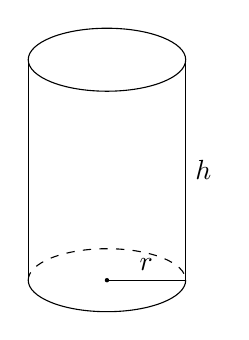
\begin{tikzpicture}[scale=0.8]
        \draw (0,0) ellipse (1.25 and 0.5);
        \draw (-1.25,0) -- (-1.25,-3.5);
        \draw (-1.25,-3.5) arc (180:360:1.25 and 0.5);
        \draw [dashed] (-1.25,-3.5) arc (180:360:1.25 and -0.5);
        \draw (1.25,-3.5) -- node[anchor=west] { $h$ } (1.25,0);  
        \draw (0, -3.5) -- node[anchor=south] { $r$ } (1.25, -3.5);
        \fill (0, -3.5) circle [radius=1pt];
    \end{tikzpicture}
\end{figure}


\subsubsection{Area}

\[
    A = 2\pi rh + 2\pi r^2 = 2\pi r(h + r),
\]


\subsubsection{Volume}

\[
    A = \pi r^2 h
\]



\subsection{Cone}

\begin{figure}[H]
    \centering
    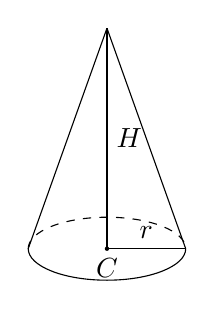
\begin{tikzpicture}[scale=0.8]
        \draw (0,0) -- (-1.25,-3.5);
        \draw (-1.25,-3.5) arc (180:360:1.25 and 0.5);
        \draw [dashed] (-1.25,-3.5) arc (180:360:1.25 and -0.5);
        \draw (1.25,-3.5) -- (0,0);  
        \draw (0,-3.5) -- node[anchor=west] { $H$ } (0,0);  
        \draw (0, -3.5) -- node[anchor=south] { $r$ } (1.25, -3.5);
        \fill (0, -3.5) circle [radius=1pt] node[anchor=north] { $C$ };
    \end{tikzpicture}
\end{figure}

\subsubsection{Area}

\[
    A = \pi r^2 + \pi r\sqrt{r^2 + H^2}
\]

\subsubsection{Volume}

\[
    V = \frac{1}{3}\pi r^2 H
\]





\subsection{Truncated Cone}

\begin{figure}[H]
  \centering 
  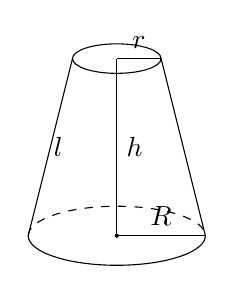
\begin{tikzpicture}[scale=0.75] % Draw top ellipse 
      \draw (0,0) ellipse (0.75 and 0.25);

      % Draw bottom ellipse
      \draw (-1.5,-3.0) arc (180:360:1.5 and 0.5);
      \draw [dashed] (-1.5,-3.0) arc (180:360:1.5 and -0.5);

      % Draw side lines
      \draw (-0.75,0) -- (-1.5,-3.0);
      \draw (1.5,-3.0) -- (0.75,0);  

      % Draw height line
      \draw (0, -3.0) -- node[midway, right] { $h$ } (0,0);  

      % Draw radii lines
      \draw (0, -3.0) -- node[midway, above] { $R$ } (1.5, -3.0);
      \draw (0, 0.0) -- node[midway, above] { $r$ } (0.75, 0.0);


      % Add labels
      \node at (-0.75, -1.5) [left] { $l$ };

      % Mark center point
      \fill (0, -3.0) circle [radius=1pt];
  \end{tikzpicture}
\end{figure}

\subsubsection{Area}

\[
  l = \sqrt(h^2 + l^2) 
\]

\[
  A  = \pi (R+r) l + \pi (R^2 + r^2)
\]

\subsubsection{Volume}

\[
    V = \frac{1}{3}\pi h(R^2 + Rr + r^2),
\]



\subsection{Angles}

What is wrong with this table ?

\begin{table}[H]
    \begin{center}
        \begin{tabular}[c]{|c|c|c|c|}
            \hline
            $\theta$ & $30^\circ$ ($\frac{\pi}{6}$) & $45^\circ$ ($\frac{\pi}{4}$) & $60^\circ$ ($\frac{\pi}{3}$) \\
            \hline
            $\sin\theta$ & $\frac{1}{2}$ & $\frac{\sqrt{2}}{2}$ & $\frac{\sqrt{3}}{2}$ \\
            \hline
            $\cos\theta$ & $\frac{\sqrt{3}}{2}$ & $\frac{\sqrt{2}}{2}$ & $\frac{1}{2}$ \\
            \hline
            $\tan\theta$ & $\frac{1}{\sqrt{3}}$ & $1$ & $\sqrt{3}$ \\
            \hline
        \end{tabular}
    \end{center}
\end{table}


\subsection{Dot product}
The dot product of vectors $\mathbf{u}$ and $\mathbf{v}$ in $n$ dimensions is given by:
\[
    \langle \mathbf{u}, \mathbf{v} \rangle = u_1 \cdot v_1 + u_2 \cdot v_2 + \ldots + u_n \cdot v_n
\]

\subsection{Magnitude}

The magnitude of a vector $\mathbf{v}$ in $n$ dimensions is given by:
\[
    |\mathbf{v}| = \sqrt{v_1^2 + v_2^2 + \ldots + v_n^2}
\]

The dot product of two Euclidean vectors $\mathbf{u}$ and $\mathbf{v}$ is defined by

\[
    \langle \mathbf{u}, \mathbf{v} \rangle = |\mathbf{u}| \cdot |\mathbf{v}| \cdot \cos(\theta)
\]


